\cleardoublepage
\phantomsection
\addcontentsline{toc}{chapter}{Введение}
\chapter*{Введение}
\label{chap:introduction}

Это --- пример оформления выпускной квалификационной работы в \LaTeX.
Набирая текст в этой системе, не нужно задумываться об оформлении документа по ГОСТу.
Требуется только разметить текст согласно структуре работы, и \LaTeX{} автоматически соберёт документ, соответствующий ГОСТу.

Обычный текст вводится так, как есть.
Отдельные предложения имеет смысл отделять друг от друга новыми строками: это помогает в редактировании, но не обязательно.
В итоговом документе такие одиночные переводы строк не учитываются.

Абзацы отделяются друг от одной или более пустыми строками.
Каждый абзац должен содержать единственную, законченную мысль.

Команды, начинающиеся с символа \verb|\|, являются специальными инструкциями \TeX{} или \LaTeX.
Чтобы оставить пробел после команды, нужно поставить фигурные скобки: \verb|\TeX{}|.

Помимо команд, также существуют окружения, использующиеся для больших блоков содержимого:
\begin{verbatim}
\begin{environment}
content
\end{environment}
\end{verbatim}

Внешние кавычки печатаются <<так>>.
Внутренние кавычки ставятся ,,так``.
Также можно использовать команду \verb|\enquote| \enquote{для автоматического \enquote{определения} уровня вложенности}.

Есть 3 основных типа тире.
Дефис \verb|-| используется для разделения сложных слов и некоторых предлогов: квадратно-гнездовой.
Короткое тире \verb|--| \en{(en-dash)} встречается в числовых диапазонах: 1970--2015.
Длинное тире \verb|---| \en{(em-dash)} --- это обычное тире в предложениях.

Для набора английского текста используйте команду \verb|\en| или окружение \verb|english|.

В данном классе и шаблоне уже настроено практически всё, что может понадобиться при написании работы.

Рисунки включаются так:
\begin{verbatim}
\begin{figure}
\centering
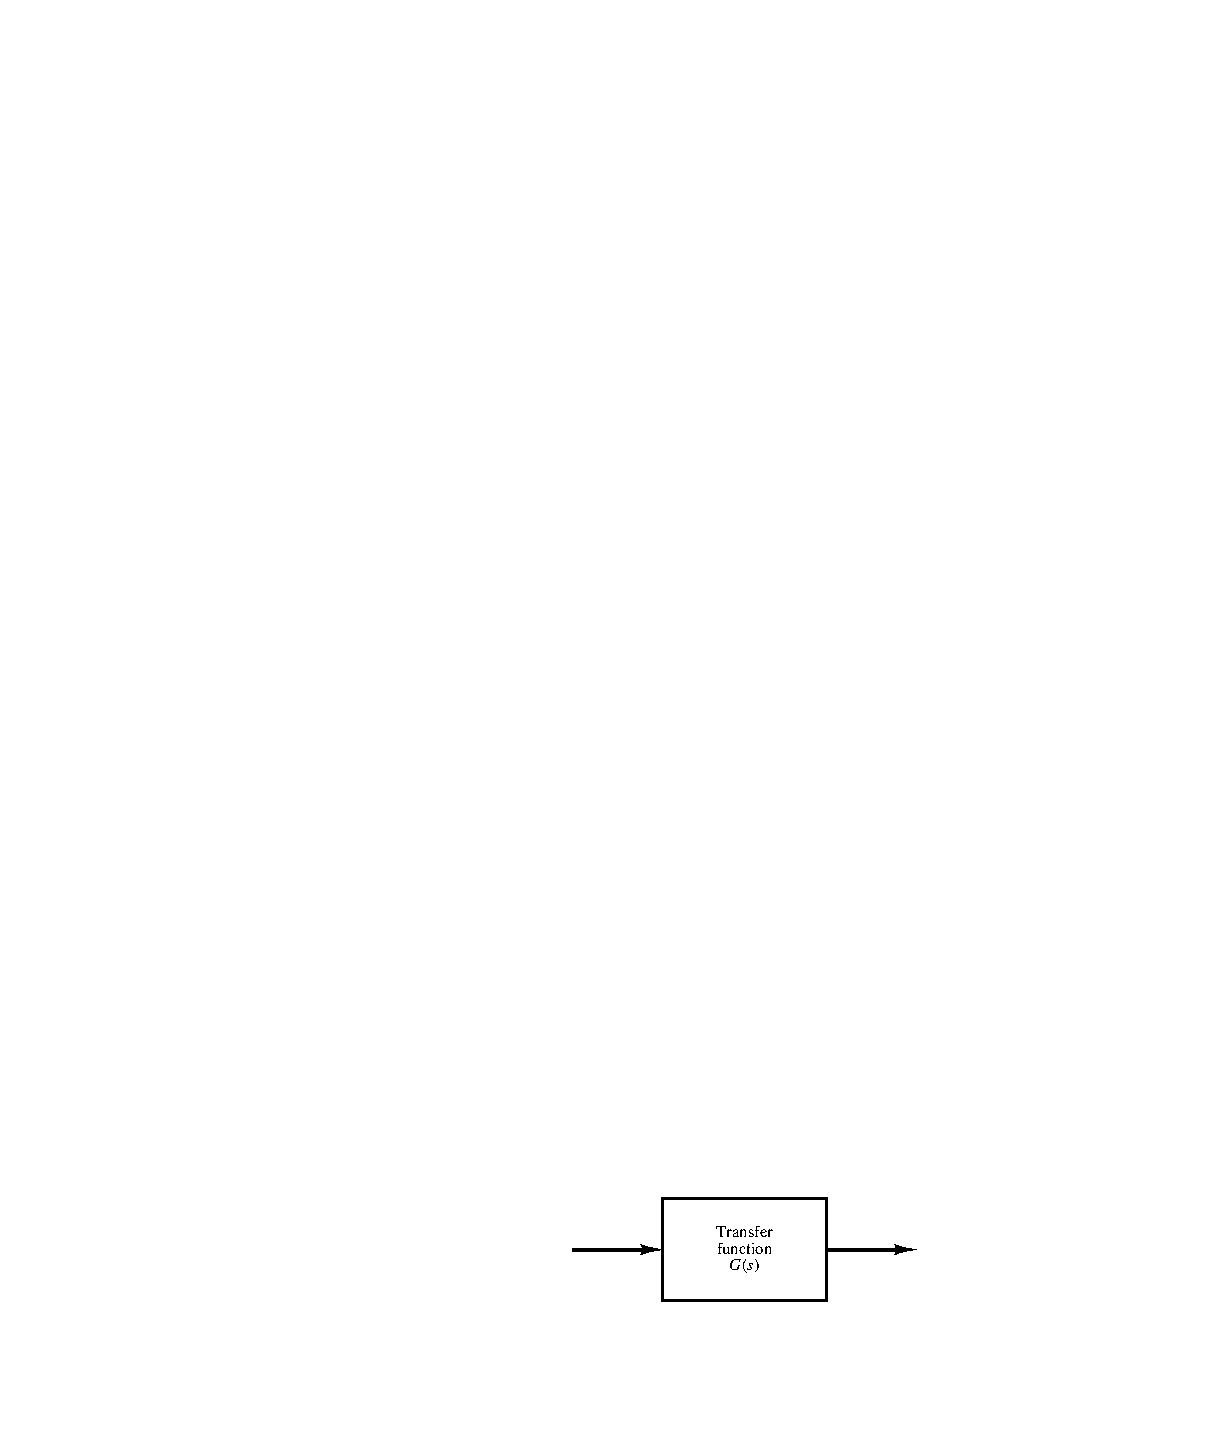
\includegraphics[width=\linewidth]{sample_figure}
\caption{Пример рисунка}
\label{fig:sample_figure}
\end{figure}
\end{verbatim}

\begin{figure}
\centering
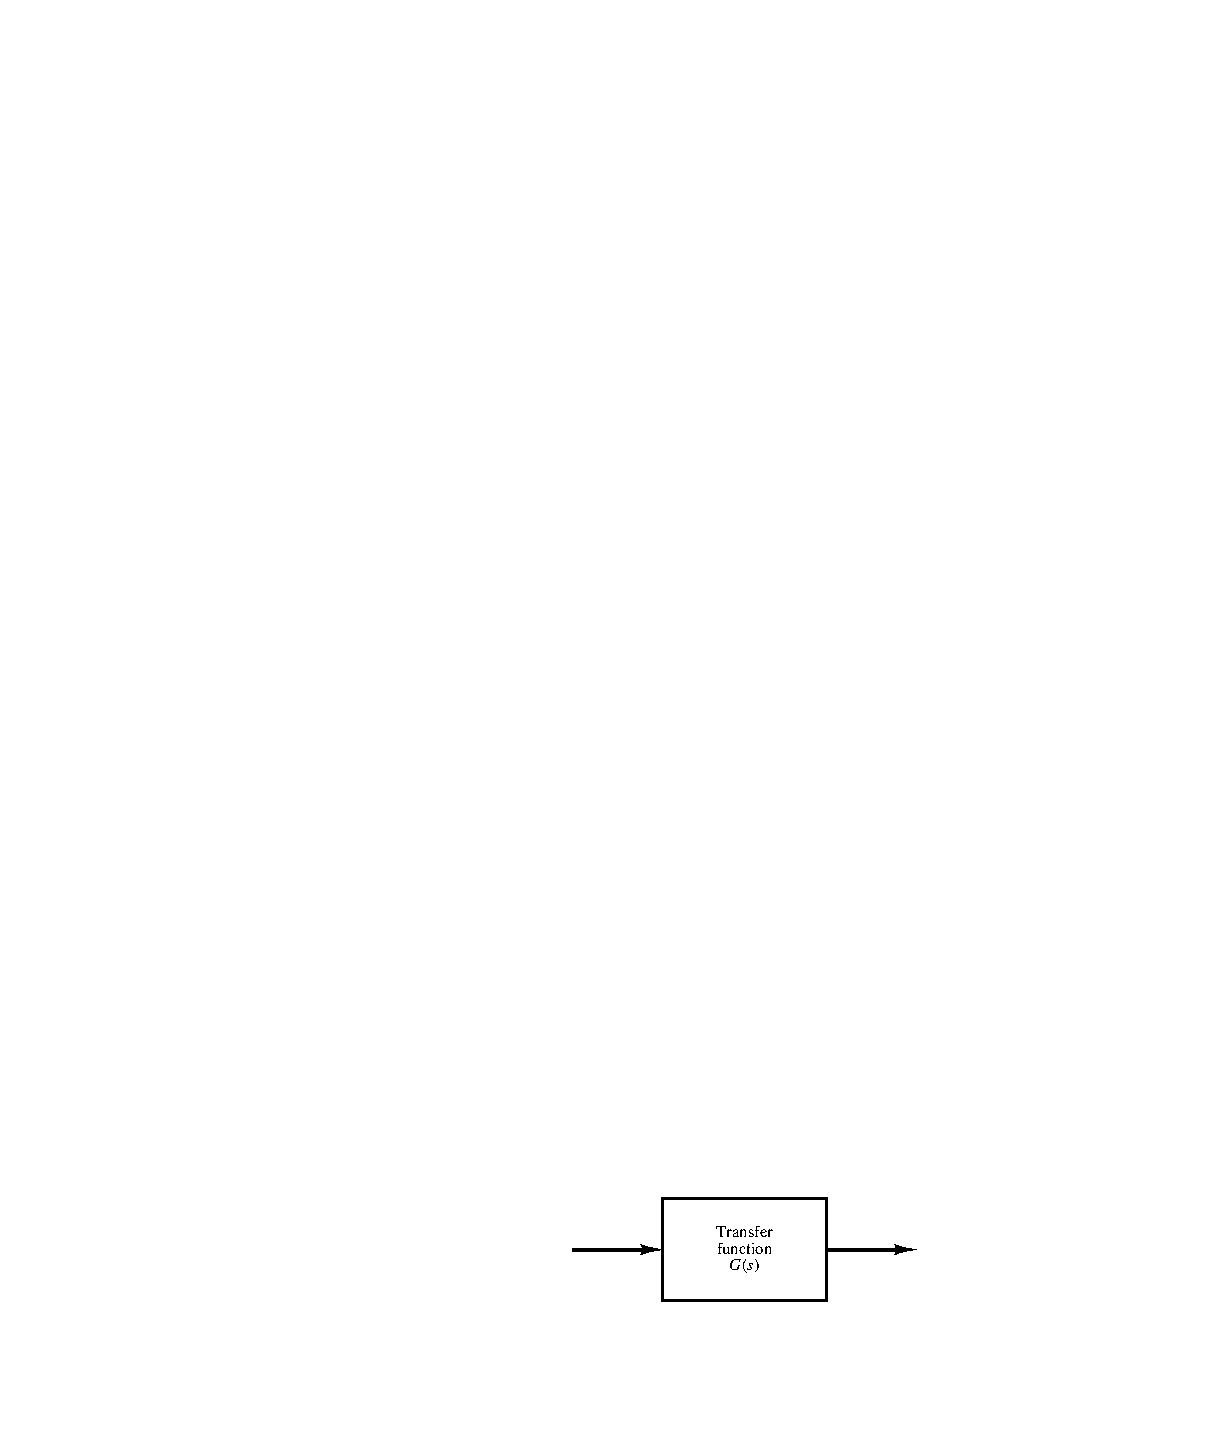
\includegraphics[width=\linewidth]{sample_figure}
\caption{Пример рисунка}
\label{fig:sample_figure}
\end{figure}

Таблицы верстаются так:
\begin{verbatim}
\begin{table}
\caption{Пример таблицы}
\label{tab:example_table}
\begin{tabular}{l c r}
\toprule
Заголовок 1 & Заголовок 2 & Заголовок 3 \\
\midrule
11 & 12 & 13 \\
21 & 22 & 23 \\
31 & 32 & 33 \\
\bottomrule
\end{tabular}
\end{table}
\end{verbatim}

\begin{table}
\caption{Пример таблицы}
\label{tab:example_table}
\begin{tabular}{l c r}
\toprule
Заголовок 1 & Заголовок 2 & Заголовок 3 \\
\midrule
11 & 12 & 13 \\
21 & 22 & 23 \\
31 & 32 & 33 \\
\bottomrule
\end{tabular}
\end{table}

Ссылаться на рисунки и таблицы можно командой \verb|\ref|: рис.~\ref{fig:sample_figure} и табл.~\ref{tab:example_table}.

Ссылки на источники создаются командой \verb|\cite|: хороший обзор возможностей \LaTeX можно найти в~\cite{oetiker1995not}.

Подробную информацию о методах работы с \LaTeX{} можно найти в Интернете.
